% !TEX root = C:/Users/piyus/knowledge/Project_Specific_Knowledge/public/fm_radio/stages/mixer/mixer.tex
\documentclass[12pt, letterpaper]{article}

\usepackage{hyperref}
\usepackage{graphicx}
\graphicspath{ {C:/Users/piyus/knowledge/Project_Specific_Knowledge/public/fm_radio/stages/mixer/pictures} }

\title{Mixer Notes}
\author{Piyush Sud}
\date{9/30/2024}
\begin{document}
\maketitle

\pagebreak

\section{High Level Design}

For the mixer, we need:

\begin{itemize}
    \item a large bandwidth (at least 200 MHz)
    \item low noise
\end{itemize}

\noindent The LT5560 works for this application. It has:

\begin{itemize}
    \item a large bandwidth (4 GHz)
    \item low noise (9.3 dB @ 900 MHz)
\end{itemize}


\noindent Design Notes:

\begin{itemize}
    \item It seems like Automatic Frequency Control (AFC) is no longer used since crystals provide a very stable frequency, as seen on both wikipedia and this link: https://www.quora.com/What-is-frequency-drift-in-an-FM-receiver. Most LOs today use digitally synthesized signals connected to crystals. These are known as "frequency synthesizers" - they are able to generate many different stable frequencies using a single reference frequency from a crystal.
    \item PLLs also don't drift because any error is compensated for in the PLL.
    \item It seems like we can just use a PLL with a VCO built in. This seems like a good option: https://www.digikey.com/en/products/detail/analog-devices-inc/ADF4360-9BCPZRL7/2043337
    \item Actually, it seems like this is an integer-N PLL, but we need a fractional N PLL.
    \item Even if we find another PLL with an integrated VCO, it seems we'll still need an external loop filter, so might as well stick with the original with an external VCO
\end{itemize}

\section{Detailed Design}

\begin{itemize}
    \item This seems like a really good PLL: \url{https://www.digikey.com/en/products/detail/skyworks-solutions-inc/SI5351A-B-GTR/4069612.} Unlike the previous one, it uses a crystal, so the frequency error is close to 0.
    \item However, it seems like it can only divide by multiples of 2, so it wouldn't work for our purposes since we need to change the LO frequency from 77 MHz to 98 MHz. 
    \item This might be a better option: \url{https://www.digikey.com/en/products/detail/analog-devices-inc/ADF4169CCPZ/5441070}
    \item In a high-side mixer, the FM modulated signal will essentially be inverted. This is because \(f_{IF} = \mid f_{RF} - f_{LO} \mid \), so if \(f_{RF}\) increases then \(f_{RF}\) becomes closer to \(f_{LO}\), so \(f_{IF}\) decreases. This doesn't really matter (not completely sure about this), as long as we're aware that it's mirrored. https://www.edaboard.com/threads/high-side-injection-and-low-side-injection-in-mixer.125131/
    \item Let's use low-side mixing so that the signal is not inverted. This means that fLO = fRF - fIF = fRF - 10.7MHz.
    \item Does a clock generator work (square wave) or do I need a sine wave for the LO?
    \item There seems to be a variety of different opinions online. \url{https://www.reddit.com/r/rfelectronics/comments/12wqxvw/rf_mixer_square_wave_lo/}
    \item It seems like a square wave is practically hard to produce, but could be beneficial. Some people are also saying that the higher order harmonics could be aliased down to the IF, others are saying that a square wave is the ideal mixer input. For now, I'm going to go with a square wave.
    \item If we're using the ADF4169CCPZ above, we'll need to write to the registers to control the input, which means we'll need a microcontroller to do that.
    \item It doesn't explicitly mention it, but looks like it uses I2C since it has a clock and data line. If not, we can just manually code the protocol instead of using an I2C library.
    \item We can use the same 0.1 uF cap we used as a blocking cap for the HF amp as a decoupling cap here since it has a very high self-resonant frequency of 6 GHz.
    \item The INT multiplier for the reference frequency is from 23 to 4095. If we want a LO signal of 77 MHz to 97 MHz, then we can potentially use a reference frequency around 1 MHz.
    \item Let's use this CMOS crystal oscillator: https://www.digikey.com/en/products/detail/analog-devices-inc-maxim-integrated/MAX7375AXR105-T/1520107
\end{itemize}

\section{Understanding PLLs}

\begin{figure}[h]
    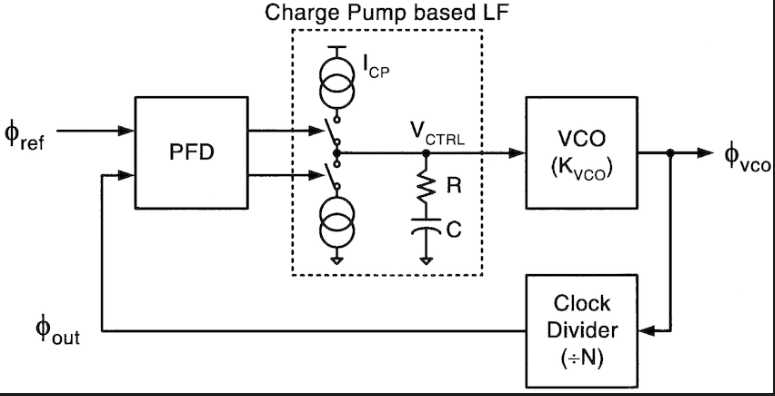
\includegraphics[width=\textwidth]{PLL_block_diagram}
\end{figure}

\begin{itemize}
    \item Assuming that the input is a square wave and the PFD is a digital circuit, a simple PFD can be implemented using an XOR gate that is high for the portion of time when the reference signal and the output signal are different. If the two signals are 1 degree out of phase, this will result in a pulse with a width of 1/180 the period of the signals.
    \item The charge pump performs integration, which can correct for both phase and freq. errors, since freq. is the derivative of phase.
    \item The charge pump for the ADF4169 outputs a current, which is converted to a voltage by the loop filter. https://electronics.stackexchange.com/questions/301056/loop-filter-of-pll
    \item Since a LPF also performs integration, a charge pump can technically replace a LPF with a capacitor.
    \item This seems like a good VCO: \url{https://www.digikey.com/en/products/detail/analog-devices-inc-maxim-integrated/MAX2623EUA-T/1938007}
\end{itemize}

\section{Loop Filter Design}

\begin{itemize}
    \item Following this link, second order loop filter design: \url{https://www.renesas.cn/cn/zh/document/apn/pll-loop-filter-design-and-fine-tuning}
    \item Desired loop bandwidth must satisfy Fpd/Fc >> 20, where Fpd is the freq. to the phase detector = the frequency of our ref signal, which is 1 MHz. This means that Fc << 1 MHz/20 = 50 kHz. Let's set the loop bandwidth to 10 kHz.
    \item Rs = \(\frac{2*pi*f_c*N}/{I_{cp}*K_{Vco}}\). N varies between 77 and 97 -> Let's choose 87 as the nominal value. According to the datasheet, it is best to start with 2.5 mA for the charge pump current. The VCO gain is given by 6.2 MHz/V. Therefore, \(Rs = \frac{2*3.1415*10000*87}{2.5*10^-3*6.2*10^6} = 352.658709677\) ohms. 
    \item Cs = \(\frac{alpha}{2*pi*f_c*R_c}\), where alpha is the ratio of the loop bandwidth to the zero frequency. It's recommended that alpha > 3, so let's do alpha = 5. That gives \(Cs = \frac{5}{2*3.1415*10000*352.6587} = 225.656757\) nF.
    \item Cp = \(\frac{Cs}{alpha*Beta}\), where beta is the ratio between pole freq. and bandwidth. It's recommended that beta > 3, so let's choose beta = 5. That gives \(Cp = \frac{225.656757*10^-9}{5*5} = 9.02627028\) nF.
    \item The maximum phase margin is given by \(arctan(\frac{b-1}{2*sqrt(b)})\), where \(b = 1 + \frac{Cs}{Cp}\). In our case, \(b = 1 + \frac{225.656757}{9.02627028} = 26\), so the phase margin = 67.80839366845 degrees \(>\) 50 degrees \(->\) the PLL is stable.
\end{itemize}

\section{Mixer Impedance Matching}

\begin{figure}[h]
    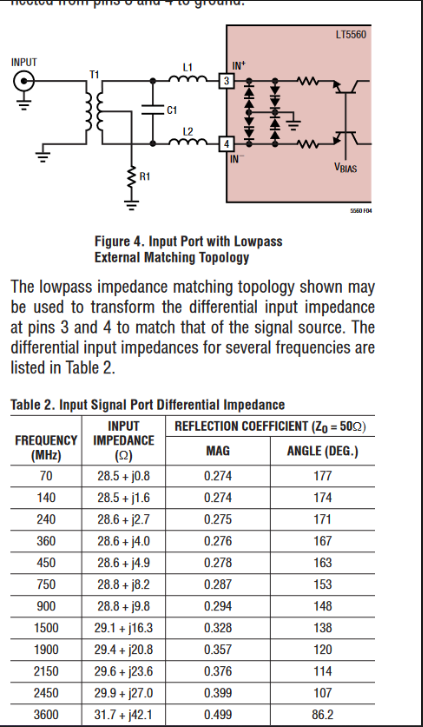
\includegraphics[width=\textwidth]{mixer_input_impedance_match}
\end{figure}

\begin{figure}[h]
    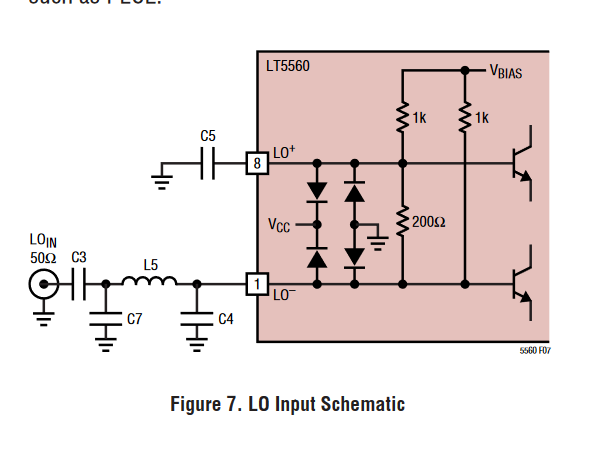
\includegraphics[width=\textwidth]{LO_circuit}
\end{figure}

\begin{figure}[h]
    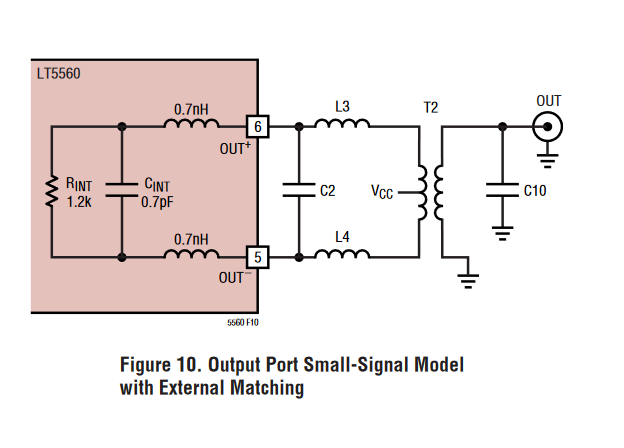
\includegraphics[width=\textwidth]{output_circuit}
\end{figure}

\begin{itemize}
    \item For the mixer, the input impedance varies between approximately 28.5 + j to 28.5 + 1.4j for the frequencies of 88 MHz to 108 MHz based on this table. 
    \item Since we're operating at a nominal frequency of 98 MHz, the input impedance = 28.5 + 1.12j. \(Q = sqrt(\frac{Rs}{Rl} - 1) = sqrt(\frac{50}{28.5} - 1) = 0.86855395049\). \(Xc = \frac{Rs}{Q} = \frac{50}{0.86855395049} = 57.5669478814 \) ohms = \( \frac{1}{2*pi*98M*C} => C = \frac{1}{2*pi*98M*57.5669478814} = 28.211154 \) pF. \( Xl = Rl*Q = 28.5*0.86855395049 = 24.753787589 \) ohms. \( X_{ext} = X_l - X_int = 24.753787589 - 1.12 = \frac{31.6931602924}{2} = 23.633787589 \) ohms. Divide this by 2 to get 11.8168937945 ohms per inductor = \(2*pi*98M*Lext => Lext = 19.1909904 \)nH.
    \item We need a transformer for converting the single ended signal to differential. We need a 1:1 ratio for impedance matching and it needs to have a center tap and operate at high frequencies. This seems like a good choice: \url{https://www.digikey.com/en/products/detail/mini-circuits/ADT1-1WT/13927938?s=N4IgTCBcDaIIIBEAqBGAtCg6kg1CAugL5A}
    \item For the LO, the datasheet gives component values in a table for some frequencies 150 MHz and above. Since the exact reactive formula is not given, we will have to extrapolate. Our LO frequency is 98 MHz - 10.7 MHz = 87.3 MHz.
    \item From the trendline, it seems like we need \(C4 = 15.443e^{-0.005*87.3} = 9.98\) pF and \(L5 = 103.57e^{0.003*87.3} = 79.71\) nH. 
    \item For the output impedance, the table gives a value for 10 MHz - that is close enough to 10.7 MHz so we can just use that, and it says that the match BW is 3 - 60 MHz for those values. At 10 MHz, it seems like the only matching needed is real, in the form of a 16:1 transformer. Let's just use the one recommended in the datasheet, as it seems like that's the one on of the only ones I can find that meets our requirements.

\end{itemize}

\begin{figure}[h]
    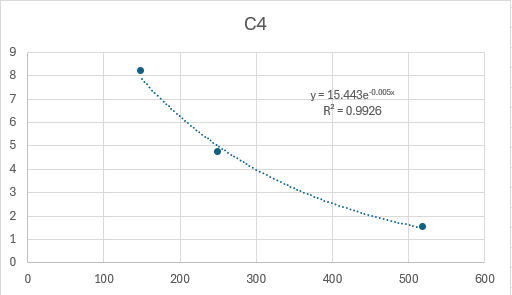
\includegraphics[width=\textwidth]{C4_trendline}
\end{figure}

\begin{figure}[h]
    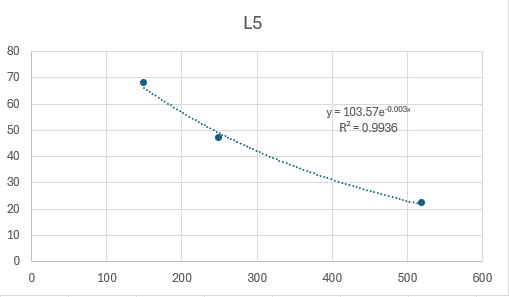
\includegraphics[width=\textwidth]{L5_trendline}
\end{figure}



\end{document}